\section{Related Work}
\label{sec:related_work}

\subsection{Racing Line calculation}
Contrary to most racing sports, where a racing line is usually drawn by an expert, video games, especially from independent developers, tend to concentrate on calculating the racing line for the computer-controlled cars.

\subsubsection{Vamos Racing Simulator}
One example is the \textit{Vamos racing simulator}\footnote{\url{http://vamos.sourceforge.net/}}. It uses an iterative cur\-va\-ture-min\-i\-mi\-za\-tion technique, simulating spring-loaded hinges that are placed in the middle of the track. The lateral forces a car produces during cornering are used to simulate the opening or closing of these hinges, iteratively shaping the racing line. After a certain number of iterations the curve stabilizes. This happens when the force across all hinges and therefore the curvature of the racing line is close to minimal. After the calculation is done, the possible speed of the racing cars at every point on the track can be calculated. 

\subsubsection{RaceOptimal}
RaceOptimal\footnote{\url{http://www.raceoptimal.com/}} is a website that offers calculated ideal racing lines for 4 different vehicles on a variety of tracks. The approach is, similarly to that of Vamos, iterative. However their focus lies on the physics of the cars. They use a Bézier-curve to approximate a smooth line across a circuit, based on predefined control points. Then the fastest possible speed for every point on the track is calculated, based on the curvature of the turn and the friction coefficient and mass of the car and limited by the cars top speed. After that the acceleration is adjusted to not exceed the power of the engine and capabilities of the tires. Lastly, the graph is adjusted to also include the capacity of the brakes and aerodynamic drag. 
This algorithm is used on a certain number of possible lines, the initial population. These solution then breed offspring, which are combinations of the initial parents, and are modified randomly, to get as many different racing lines as possible.
The best children are kept and breed again, bad solutions will be thrown away. This process is repeated until the result, being the lap time on the given track, stays consistently quick.

A similar genetic approach is used in this paper: \cite{cardamone10}. Here the track is decomposed into several segments and for each segment a algorithm is applied, that searches the best trade-off between the minimization of the length and curvature of the racing line. To assess the fitness of each genetic iteration, the solution is tested in the TORCS racing simulator\footnote{\url{https://sourceforge.net/projects/torcs/}}.

\subsubsection{Optimal Control}
Optimal control is an optimization method that, in general, tries to minimize a cost function of control variables in a dynamic system. In case of racing line optimization, the cost function is the lap time, the control variables are steering angle and throttle/break input and the dynamic system is a vehicle model restricted to the boundaries of the road. \cite{gustafsson08,brayshaw05}

\subsubsection{Euler Spiral Method}
An Euler spiral (figure \ref{fig:euler_spiral}) is a curve whose curvature changes linearly with its curve length. They can be used to connect a tangent to a circular curve, which can be translated to connecting a straight with a curve on a track.\\ \cite{xiong09}

\begin{figure}[!ht]
	\centering
	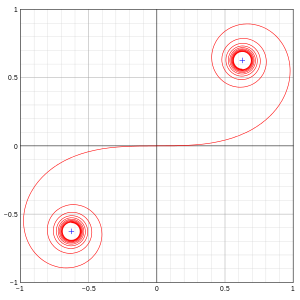
\includegraphics[width=.5\textwidth]{euler_spiral}
	\caption{A double-ended Euler spiral}
	\label{fig:euler_spiral}
\end{figure}

The racing line follows a segment of the Euler spiral that connects a starting point with an end point. This come close to minimizing the curvature, but does not completely reach the minimum. Also there are multiple segments that connect two points, so as, usually, the least curvature is wanted, the segment with the biggest radius is taken.

Most of these methods either need exact knowledge of the track or a simulation to work. This paper discusses possibilities to compare racing lines on an arbitrary track with no additional software other than a web browser.

\clearpage